\documentclass[final]{beamer}
\usepackage[orientation=portrait,size=a0,scale=1.0]{beamerposter}
\usepackage[T1]{fontenc}
\usepackage[utf8]{inputenc}
\usepackage[scaled=0.92]{helvet}
\renewcommand{\familydefault}{\sfdefault}
\usepackage{graphicx}
\usepackage{amsmath,amssymb}
\usepackage{booktabs}
\usepackage{tcolorbox}
\tcbuselibrary{skins,breakable}
\usepackage{ragged2e}
\usepackage{xcolor}
\usepackage{tikz}
\usetikzlibrary{arrows.meta,positioning,calc}
\usepackage{hyperref}

\graphicspath{{figures/}}

\definecolor{posterNavy}{HTML}{0B1F33}
\definecolor{posterTeal}{HTML}{008C95}
\definecolor{posterOrange}{HTML}{E77C2B}
\definecolor{posterAmber}{HTML}{F2C14E}
\definecolor{posterSurface}{HTML}{F2F6F8}
\definecolor{posterBlueSurface}{HTML}{E6F1F4}
\definecolor{posterInk}{HTML}{17212B}
\definecolor{posterMuted}{HTML}{4E5D68}
\definecolor{posterGreen}{HTML}{1E7A63}
\definecolor{posterRed}{HTML}{B94736}

\setbeamertemplate{navigation symbols}{}
\setbeamertemplate{frametitle}{}
\setbeamercolor{normal text}{fg=posterInk,bg=white}
\setbeamercolor{structure}{fg=posterNavy}
\setbeamersize{text margin left=2.25cm,text margin right=2.25cm}
\setlength{\parindent}{0pt}
\setlength{\parskip}{0.30em}
\sloppy

\newcommand{\body}{\fontsize{29}{36}\selectfont}
\newcommand{\bodylarge}{\fontsize{33}{40}\selectfont}
\newcommand{\captionfont}{\fontsize{26}{31}\selectfont}
\newcommand{\smallfont}{\fontsize{23}{28}\selectfont}
\newcommand{\sectiontitle}[2]{\color{#1}\fontsize{54}{62}\selectfont\bfseries #2\par}
\newcommand{\subhead}[2]{\color{#1}\fontsize{31}{37}\selectfont\bfseries #2\par}
\newcommand{\metric}[4]{%
  \begin{minipage}[t]{0.30\linewidth}\centering
    {\color{#1}\fontsize{91}{96}\selectfont\bfseries #2\par}
    {\color{posterMuted}\fontsize{27}{33}\selectfont #3\par}
    {\color{#4}\rule{0.84\linewidth}{2.7pt}\par}
  \end{minipage}%
}
\newcommand{\bulletline}[2]{\textcolor{#1}{\fontsize{31}{37}\selectfont\bfseries\textbullet}\hspace{0.18cm}{\body #2}\par}

\begin{document}
\begin{frame}[t]

% ------------------------------------------------------------------
% TITLE
% ------------------------------------------------------------------
\begin{tcolorbox}[enhanced,colback=posterNavy,colframe=posterNavy,boxrule=0pt,
  arc=0pt,left=0.72cm,right=0.72cm,top=0.38cm,bottom=0.38cm]
  {\color{white}\fontsize{70}{78}\selectfont\bfseries
  Feasibility Assessment of Balanced-Model EV Charging-Flexibility\\[-0.02em]
  Schedules in Unbalanced Three-Phase Distribution Networks\par}
  \vspace{0.16cm}
  {\color{posterAmber}\fontsize{37}{44}\selectfont\bfseries
  A balanced-model flexibility offer is a plan, not yet a dispatchable product.\par}
  \vspace{0.10cm}
  {\color{white}\fontsize{31}{37}\selectfont
  Validate the fixed vehicle--time allocation on the detailed feeder, then return the largest safe fraction $\alpha^*$ before dispatch.\par}
  \vspace{0.16cm}
  {\color{white}\fontsize{28}{34}\selectfont
  Junxing Tan \quad Jun Wu \quad Shiting Cui \quad Chaofan Yang \quad Jiangcheng Wang\quad
  \textit{Wuhan University}\hfill IEEE PES ISGT Asia 2026 \quad Paper ID 9499\par}
\end{tcolorbox}

\vspace{0.22cm}

% ------------------------------------------------------------------
% BLOCK 1: WHY IT MATTERS
% ------------------------------------------------------------------
\begin{tcolorbox}[enhanced,colback=posterSurface,colframe=posterOrange,boxrule=2.3pt,
  arc=6pt,left=0.65cm,right=0.65cm,top=0.34cm,bottom=0.34cm]
  \sectiontitle{posterOrange}{1\quad Why balanced offers can fail}
  \begin{minipage}[t]{0.32\linewidth}\vspace{0pt}
    \subhead{posterNavy}{The implementation gap}
    {\body
    EV flexibility is often planned with a balanced or aggregate network model. After the original feeder phases, EV locations, and load imbalance are restored, the same vehicle-level V1G schedule can exceed voltage, VUF, transformer, or feeder-head limits.\par}
  \end{minipage}\hfill
  \begin{minipage}[t]{0.32\linewidth}\vspace{0pt}
    \subhead{posterOrange}{The question}
    {\color{posterNavy}\bodylarge\bfseries
    How much of a fixed vehicle-level offer can be dispatched safely?\par}
    \vspace{0.20cm}
    {\body
    The goal is not to redesign which EV charges when. It is to quantify the network headroom left in an already computed schedule.\par}
  \end{minipage}\hfill
  \begin{minipage}[t]{0.32\linewidth}\vspace{0pt}
    \subhead{posterTeal}{The output}
    {\body
    For every case, the procedure returns two operational quantities:\par}
    \bulletline{posterTeal}{the largest verified feasible factor $\alpha^*\in[0,1]$;}
    \bulletline{posterTeal}{the first network constraint that blocks a larger offer.}
    \vspace{0.10cm}
    {\color{posterMuted}\smallfont\itshape Evidence below covers 46 evaluated scenarios on two benchmark feeders; it is case-study evidence, not a universal guarantee.\par}
  \end{minipage}
\end{tcolorbox}

\vspace{0.22cm}

% ------------------------------------------------------------------
% BLOCK 2: METHOD
% ------------------------------------------------------------------
\begin{tcolorbox}[enhanced,colback=posterBlueSurface,colframe=posterTeal,boxrule=2.3pt,
  arc=6pt,left=0.65cm,right=0.65cm,top=0.34cm,bottom=0.34cm]
  \sectiontitle{posterTeal}{2\quad From a planned schedule to a safe dispatch}
  {\color{posterMuted}\body
  The schedule-preserving gate keeps the original EV--time pattern and changes only its implementation level. Vehicle feasibility is inherited from the two endpoints under the continuous V1G model; network feasibility is re-tested in the detailed unbalanced feeder.\par}
  \vspace{0.16cm}
  \begin{center}
  \begin{tikzpicture}[
    flow/.style={rounded corners=5pt,draw=posterTeal,fill=white,line width=1.5pt,
      text width=0.165\linewidth,minimum height=1.80cm,align=left,inner xsep=0.25cm,
      inner ysep=0.15cm,font=\fontsize{24}{29}\selectfont},
    arrow/.style={-Latex,line width=2.2pt,draw=posterOrange}
  ]
    \node[flow] (a) {\textcolor{posterTeal}{\bfseries 1\\Baseline}\\availability, energy demand, charging limits};
    \node[flow,right=0.28cm of a] (b) {\textcolor{posterTeal}{\bfseries 2\\Target}\\balanced-model vehicle-level V1G schedule};
    \node[flow,right=0.28cm of b] (c) {\textcolor{posterTeal}{\bfseries 3\\Scale}\\$u(\alpha)=u^0+\alpha(u^B-u^0)$};
    \node[flow,right=0.28cm of c] (d) {\textcolor{posterTeal}{\bfseries 4\\Check}\\96-slot nonlinear three-phase power flow};
    \node[flow,right=0.28cm of d] (e) {\textcolor{posterTeal}{\bfseries 5\\Return}\\largest passing $\alpha^*$ + first limit};
    \draw[arrow] (a) -- (b); \draw[arrow] (b) -- (c); \draw[arrow] (c) -- (d); \draw[arrow] (d) -- (e);
  \end{tikzpicture}
  \end{center}
  \vspace{0.18cm}
  \begin{minipage}[t]{0.58\linewidth}\vspace{0pt}
    \begin{tcolorbox}[colback=white,colframe=posterNavy,boxrule=1.5pt,arc=4pt,
      left=0.35cm,right=0.35cm,top=0.20cm,bottom=0.20cm]
      \centering
      {\color{posterNavy}\fontsize{45}{52}\selectfont\bfseries
      $u_{i,t}(\alpha)=u^0_{i,t}+\alpha\bigl(u^B_{i,t}-u^0_{i,t}\bigr),\quad 0\le\alpha\le1$\par}
      {\color{posterMuted}\captionfont Both endpoints satisfy availability, power bounds, cumulative-energy, and departure-target constraints; intermediate continuous V1G schedules preserve the same vehicle--time allocation.\par}
    \end{tcolorbox}
  \end{minipage}\hfill
  \begin{minipage}[t]{0.38\linewidth}\vspace{0pt}
    \subhead{posterOrange}{Network gate at every 15-min slot}
    \bulletline{posterOrange}{$0.95\le V\le1.06$ p.u.}
    \bulletline{posterOrange}{VUF $\le2\%$}
    \bulletline{posterOrange}{transformer loading $\le1.0$ p.u.}
    \bulletline{posterOrange}{feeder-head loading $\le1.0$ p.u.}
  \end{minipage}
  \vspace{0.16cm}
  \begin{tcolorbox}[colback=posterNavy,colframe=posterNavy,boxrule=0pt,arc=4pt,
    left=0.35cm,right=0.35cm,top=0.18cm,bottom=0.18cm]
    {\color{posterAmber}\fontsize{31}{37}\selectfont\bfseries How to read $\alpha^*$:\hspace{0.20cm}}
    {\color{white}\body If $\alpha^*=1$, the target is fully dispatchable. If $\alpha^*=0.54$, dispatch 54\% of the original adjustment while keeping the same EV--time pattern; the remaining 46\% is withheld at the first feeder limit.\par}
  \end{tcolorbox}
\end{tcolorbox}

\vspace{0.22cm}

% ------------------------------------------------------------------
% BLOCK 3: STUDY DESIGN
% ------------------------------------------------------------------
\begin{tcolorbox}[enhanced,colback=white,colframe=posterNavy,boxrule=2.3pt,
  arc=6pt,left=0.65cm,right=0.65cm,top=0.34cm,bottom=0.34cm]
  \sectiontitle{posterNavy}{3\quad Study design}
  \begin{minipage}[t]{0.34\linewidth}\vspace{0pt}\centering
    {\color{posterTeal}\fontsize{31}{37}\selectfont\bfseries Restore the feeder detail\par}
    \vspace{0.08cm}
    \begin{minipage}[t]{0.48\linewidth}\centering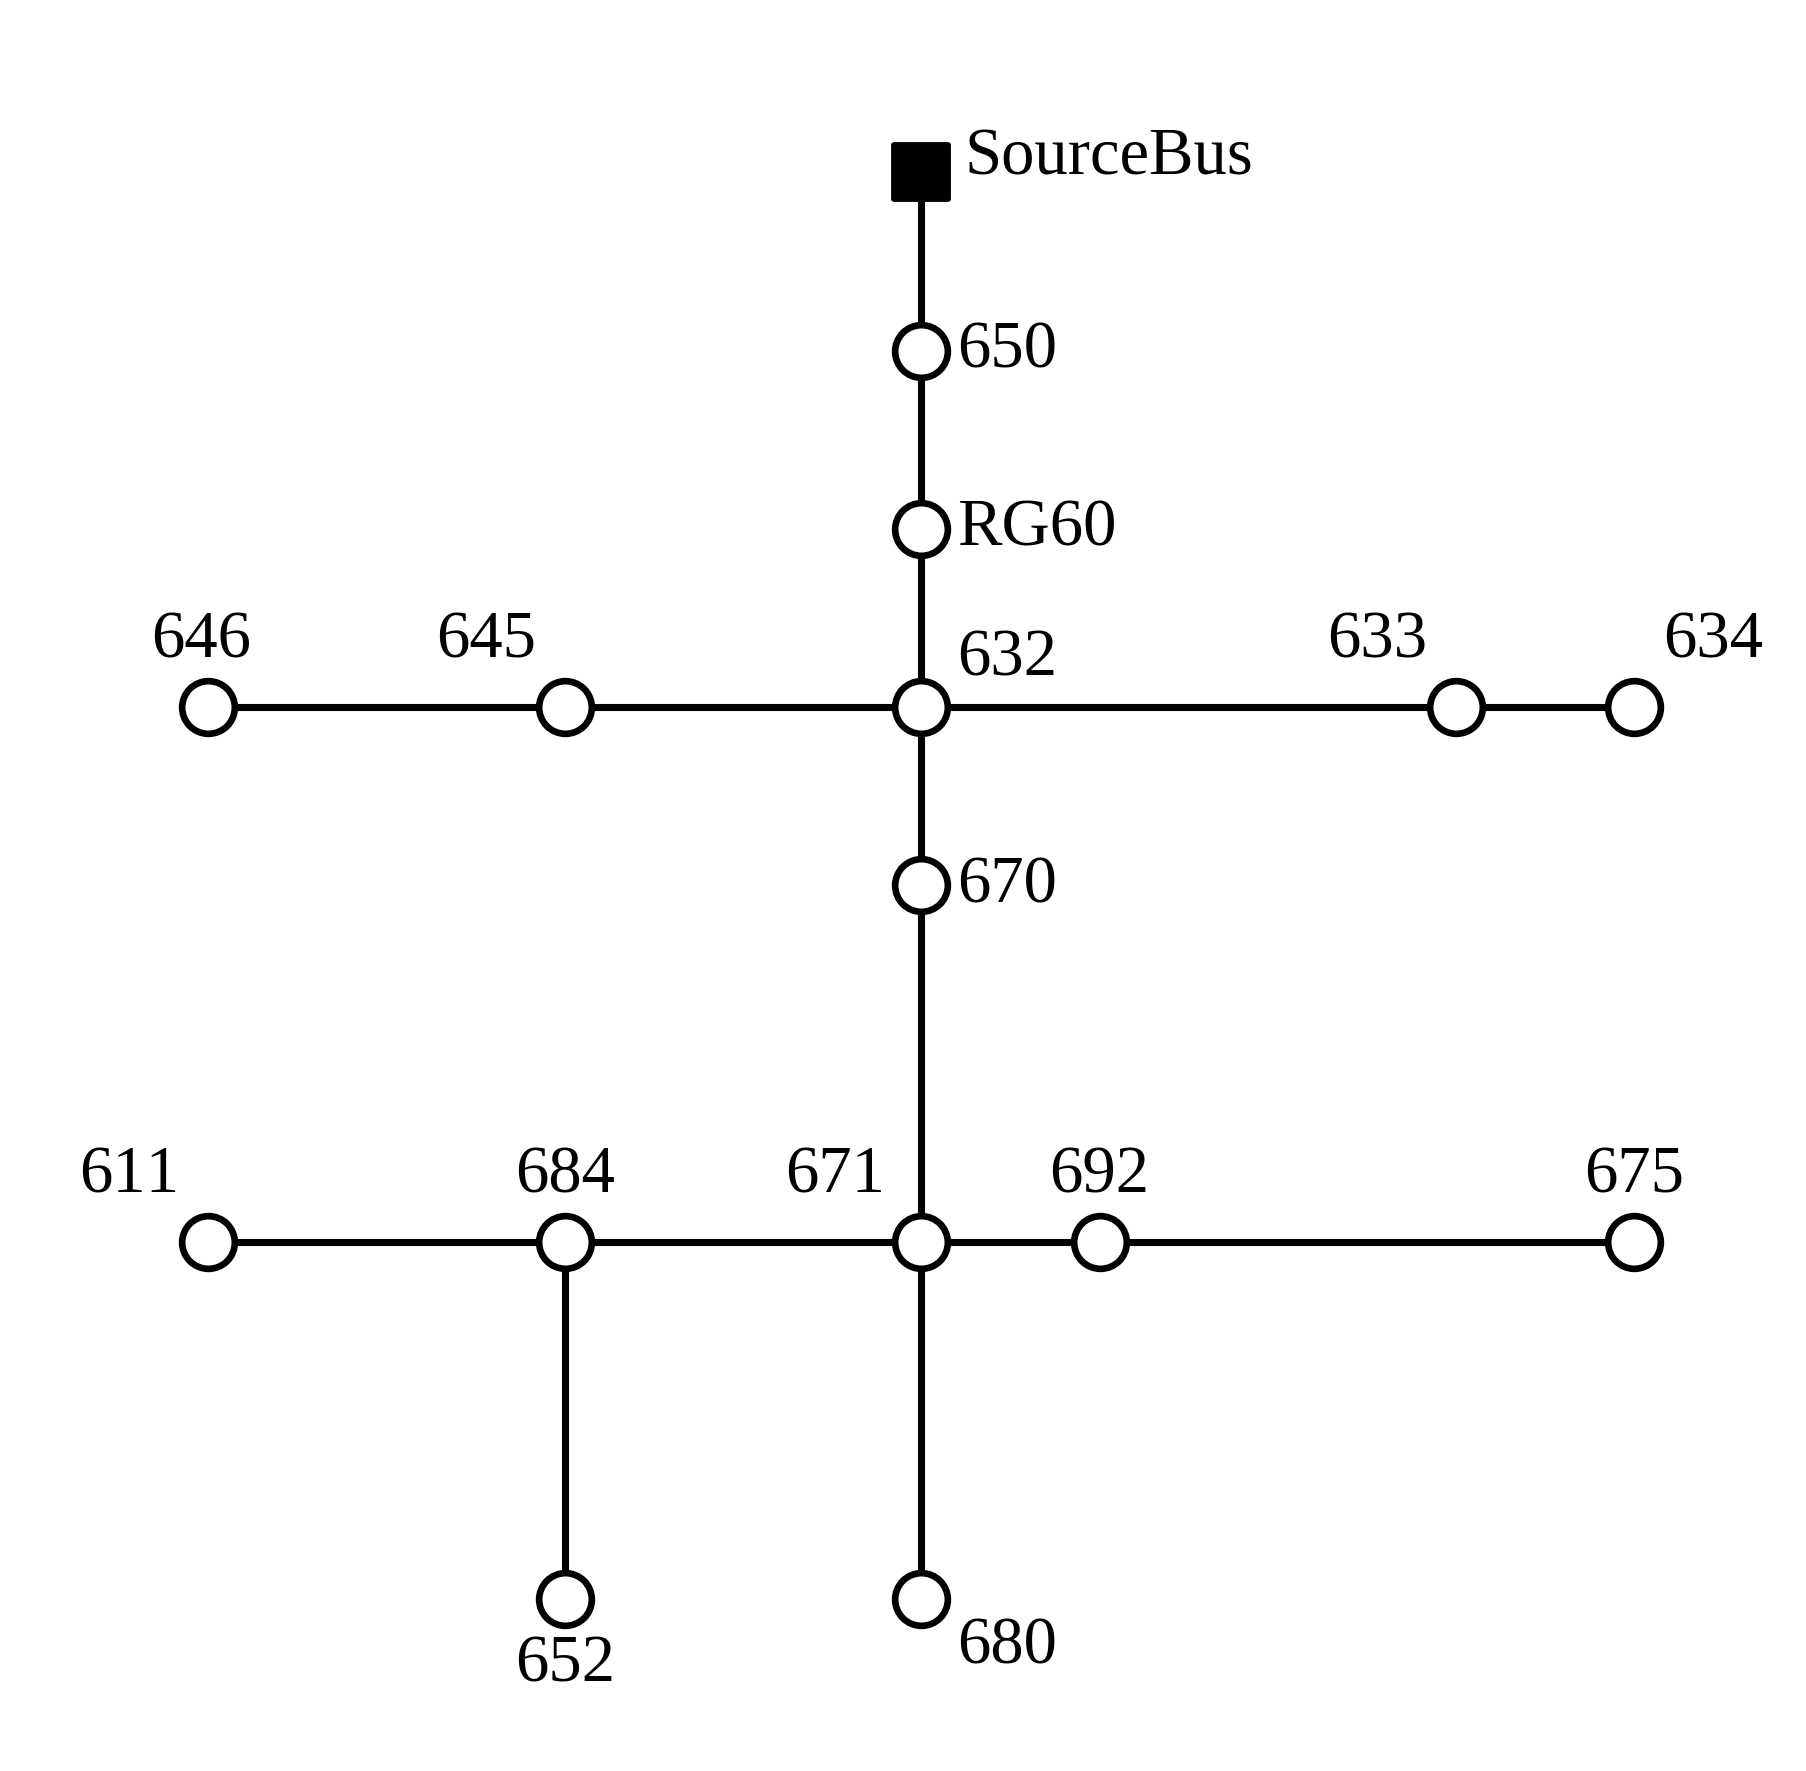
\includegraphics[height=5.0cm,keepaspectratio]{fig2a_ieee13_topology.png}\\[-0.02cm]{\captionfont\bfseries IEEE13}\end{minipage}\hfill
    \begin{minipage}[t]{0.48\linewidth}\centering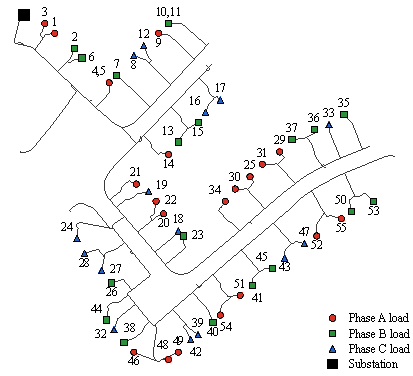
\includegraphics[height=5.0cm,keepaspectratio]{fig2b_lv906_topology.pdf}\\[-0.02cm]{\captionfont\bfseries LV906}\end{minipage}
    \vspace{0.08cm}
    {\color{posterMuted}\body OpenDSS validation restores phase assignments, feeder imbalance, and EV connection points before the three-phase check.\par}
  \end{minipage}\hfill
  \begin{minipage}[t]{0.31\linewidth}\vspace{0pt}
    {\color{posterOrange}\fontsize{31}{37}\selectfont\bfseries Case matrix\par}
    {\color{posterNavy}\fontsize{66}{72}\selectfont\bfseries 22 + 24 = 46\par}
    {\color{posterMuted}\body IEEE13 + LV906 evaluated cases.\par}
    \vspace{0.06cm}
    {\color{posterNavy}\fontsize{48}{54}\selectfont\bfseries 96$\times$501\par}
    {\color{posterMuted}\body quarter-hour slots $\times$ candidate $\alpha$ values per case.\par}
    \vspace{0.06cm}
    {\body Four call times: 00:00, 02:00, 06:00, and 19:00; six EV realizations per feeder--call-time pair.\par}
    \vspace{0.08cm}
    {\color{posterMuted}\smallfont EV inputs are sampled from 3,568 NHTS vehicle-day records.\par}
  \end{minipage}\hfill
  \begin{minipage}[t]{0.31\linewidth}\vspace{0pt}
    {\color{posterGreen}\fontsize{31}{37}\selectfont\bfseries Feeder comparison\par}
    \vspace{0.10cm}
    \renewcommand{\arraystretch}{1.35}
    \setlength{\tabcolsep}{0.16cm}
    {\fontsize{24}{30}\selectfont
    \begin{tabular}{lrrrr}
      \toprule
      & cases & mean $\alpha^*$ & median & full\\
      \midrule
      IEEE13 & 22 & 0.834 & 0.999 & 11/22\\
      LV906  & 24 & 0.540 & 0.446 & 3/24\\
      Overall& 46 & 0.681 & 0.719 & 14/46\\
      \bottomrule
    \end{tabular}\par}
    \vspace{0.16cm}
    {\color{posterMuted}\body
    A full result means $\alpha^*=1$. The study deliberately compares a small meshed benchmark with a larger low-voltage feeder where phase imbalance has more room to accumulate.\par}
  \end{minipage}
  \vspace{0.16cm}
  \begin{tcolorbox}[colback=posterBlueSurface,colframe=posterTeal,boxrule=1.4pt,arc=4pt,
    left=0.35cm,right=0.35cm,top=0.18cm,bottom=0.18cm]
    \centering
    {\color{posterNavy}\bodylarge\bfseries The validation is schedule-specific: each candidate must pass every active constraint at every time slot before it is called dispatchable.\par}
  \end{tcolorbox}
\end{tcolorbox}

\vspace{0.22cm}

% ------------------------------------------------------------------
% BLOCK 4: RESULTS
% ------------------------------------------------------------------
\begin{tcolorbox}[enhanced,colback=posterSurface,colframe=posterOrange,boxrule=2.3pt,
  arc=6pt,left=0.65cm,right=0.65cm,top=0.34cm,bottom=0.34cm]
  \sectiontitle{posterOrange}{4\quad What changes at dispatch?}
  {\color{posterInk}\bodylarge
  The balanced target is often only partially deliverable. Derating is not a change in the EV pattern: it is a network-feasibility correction applied before the offer reaches dispatch.\par}
  \vspace{0.12cm}
  \begin{center}
    \metric{posterNavy}{32/46}{target schedules require derating}{posterOrange}\hfill
    \metric{posterOrange}{14/46}{fully implementable at $\alpha^*=1$}{posterGreen}\hfill
    \metric{posterTeal}{27/32}{limited cases first blocked by voltage or VUF}{posterTeal}
  \end{center}
  \vspace{0.18cm}\hrule\vspace{0.20cm}
  \begin{minipage}[t]{0.45\linewidth}\vspace{0pt}\centering
    {\color{posterTeal}\fontsize{33}{39}\selectfont\bfseries Verified scaling factors\par}
    \vspace{0.06cm}
    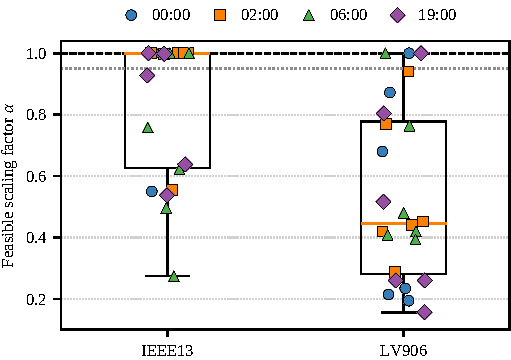
\includegraphics[height=17.5cm,keepaspectratio]{fig4_feasible_scaling_distribution.pdf}\\[-0.02cm]
    {\color{posterMuted}\captionfont IEEE13 retains more headroom (mean $\alpha^*=0.834$) than LV906 (mean $\alpha^*=0.540$).\par}
  \end{minipage}\hfill
  \begin{minipage}[t]{0.30\linewidth}\vspace{0pt}\centering
    {\color{posterOrange}\fontsize{33}{39}\selectfont\bfseries First limiting constraint\par}
    \vspace{0.06cm}
    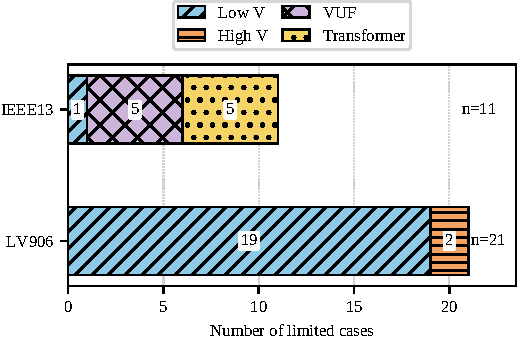
\includegraphics[height=12.5cm,keepaspectratio]{fig5_limiting_network_constraints.pdf}\\[-0.02cm]
    {\color{posterMuted}\captionfont Voltage magnitude or VUF is the first limit in 27 of the 32 derated cases.\par}
  \end{minipage}\hfill
  \begin{minipage}[t]{0.22\linewidth}\vspace{0pt}
    {\color{posterNavy}\fontsize{31}{37}\selectfont\bfseries Why it matters\par}
    {\body
    Similar scheduled offers can yield different verified offers because phase imbalance and network headroom differ.\par}
    \vspace{0.12cm}
    {\color{posterTeal}\fontsize{29}{35}\selectfont\bfseries How to read the offer\par}
    \begin{tcolorbox}[colback=white,colframe=posterTeal,boxrule=1.3pt,arc=3pt,left=0.22cm,right=0.22cm,top=0.12cm,bottom=0.12cm]
      {\color{posterNavy}\fontsize{29}{34}\selectfont\bfseries $\alpha^*=1.00$}\quad {\body 100\% of the planned adjustment is dispatchable.}\par
      \vspace{0.05cm}
      {\color{posterTeal}\fontsize{29}{34}\selectfont\bfseries $\alpha^*=0.54$}\quad {\body 54\% is dispatchable; 46\% is withheld at the first limit.}\par
    \end{tcolorbox}
    \vspace{0.10cm}
    {\color{posterRed}\fontsize{28}{34}\selectfont\bfseries LV906: 21/24 cases are limited; 19 by low voltage and 2 by high voltage.\par}
  \end{minipage}
  \vspace{0.20cm}
  \begin{tcolorbox}[colback=posterNavy,colframe=posterNavy,boxrule=0pt,arc=4pt,
    left=0.35cm,right=0.35cm,top=0.20cm,bottom=0.20cm]
    {\color{posterAmber}\fontsize{34}{40}\selectfont\bfseries Operational message\hspace{0.25cm}}
    {\color{white}\bodylarge Validate $\rightarrow$ derate $\rightarrow$ dispatch. The procedure preserves the original vehicle--time allocation while making feeder headroom explicit; rerun it when feeder or EV states change.\par}
  \end{tcolorbox}
  \vspace{0.10cm}
  {\color{posterMuted}\smallfont\itshape Evidence from 46 evaluated scenarios; the first limiting constraint is scenario-specific.\hfill\href{https://github.com/Kato814/EV-FLEX-BIAS}{github.com/Kato814/EV-FLEX-BIAS}\par}
\end{tcolorbox}

\end{frame}
\end{document}



